\documentclass[1p]{elsarticle_modified}
%\bibliographystyle{elsarticle-num}

%\usepackage[colorlinks]{hyperref}
%\usepackage{abbrmath_seonhwa} %\Abb, \Ascr, \Acal ,\Abf, \Afrak
\usepackage{amsfonts}
\usepackage{amssymb}
\usepackage{amsmath}
\usepackage{amsthm}
\usepackage{scalefnt}
\usepackage{amsbsy}
\usepackage{kotex}
\usepackage{caption}
\usepackage{subfig}
\usepackage{color}
\usepackage{graphicx}
\usepackage{xcolor} %% white, black, red, green, blue, cyan, magenta, yellow
\usepackage{float}
\usepackage{setspace}
\usepackage{hyperref}

\usepackage{tikz}
\usetikzlibrary{arrows}

\usepackage{multirow}
\usepackage{array} % fixed length table
\usepackage{hhline}

%%%%%%%%%%%%%%%%%%%%%
\makeatletter
\renewcommand*\env@matrix[1][\arraystretch]{%
	\edef\arraystretch{#1}%
	\hskip -\arraycolsep
	\let\@ifnextchar\new@ifnextchar
	\array{*\c@MaxMatrixCols c}}
\makeatother %https://tex.stackexchange.com/questions/14071/how-can-i-increase-the-line-spacing-in-a-matrix
%%%%%%%%%%%%%%%

\usepackage[normalem]{ulem}

\newcommand{\msout}[1]{\ifmmode\text{\sout{\ensuremath{#1}}}\else\sout{#1}\fi}
%SOURCE: \msout is \stkout macro in https://tex.stackexchange.com/questions/20609/strikeout-in-math-mode

\newcommand{\cancel}[1]{
	\ifmmode
	{\color{red}\msout{#1}}
	\else
	{\color{red}\sout{#1}}
	\fi
}

\newcommand{\add}[1]{
	{\color{blue}\uwave{#1}}
}

\newcommand{\replace}[2]{
	\ifmmode
	{\color{red}\msout{#1}}{\color{blue}\uwave{#2}}
	\else
	{\color{red}\sout{#1}}{\color{blue}\uwave{#2}}
	\fi
}

\newcommand{\Sol}{\mathcal{S}} %segment
\newcommand{\D}{D} %diagram
\newcommand{\A}{\mathcal{A}} %arc


%%%%%%%%%%%%%%%%%%%%%%%%%%%%%5 test

\def\sl{\operatorname{\textup{SL}}(2,\Cbb)}
\def\psl{\operatorname{\textup{PSL}}(2,\Cbb)}
\def\quan{\mkern 1mu \triangleright \mkern 1mu}

\theoremstyle{definition}
\newtheorem{thm}{Theorem}[section]
\newtheorem{prop}[thm]{Proposition}
\newtheorem{lem}[thm]{Lemma}
\newtheorem{ques}[thm]{Question}
\newtheorem{cor}[thm]{Corollary}
\newtheorem{defn}[thm]{Definition}
\newtheorem{exam}[thm]{Example}
\newtheorem{rmk}[thm]{Remark}
\newtheorem{alg}[thm]{Algorithm}

\newcommand{\I}{\sqrt{-1}}
\begin{document}

%\begin{frontmatter}
%
%\title{Boundary parabolic representations of knots up to 8 crossings}
%
%%% Group authors per affiliation:
%\author{Yunhi Cho} 
%\address{Department of Mathematics, University of Seoul, Seoul, Korea}
%\ead{yhcho@uos.ac.kr}
%
%
%\author{Seonhwa Kim} %\fnref{s_kim}}
%\address{Center for Geometry and Physics, Institute for Basic Science, Pohang, 37673, Korea}
%\ead{ryeona17@ibs.re.kr}
%
%\author{Hyuk Kim}
%\address{Department of Mathematical Sciences, Seoul National University, Seoul 08826, Korea}
%\ead{hyukkim@snu.ac.kr}
%
%\author{Seokbeom Yoon}
%\address{Department of Mathematical Sciences, Seoul National University, Seoul, 08826,  Korea}
%\ead{sbyoon15@snu.ac.kr}
%
%\begin{abstract}
%We find all boundary parabolic representation of knots up to 8 crossings.
%
%\end{abstract}
%\begin{keyword}
%    \MSC[2010] 57M25 
%\end{keyword}
%
%\end{frontmatter}

%\linenumbers
%\tableofcontents
%
\newcommand\colored[1]{\textcolor{white}{\rule[-0.35ex]{0.8em}{1.4ex}}\kern-0.8em\color{red} #1}%
%\newcommand\colored[1]{\textcolor{white}{ #1}\kern-2.17ex	\textcolor{white}{ #1}\kern-1.81ex	\textcolor{white}{ #1}\kern-2.15ex\color{red}#1	}

{\Large $\underline{12n_{0578}~(K12n_{0578})}$}

\setlength{\tabcolsep}{10pt}
\renewcommand{\arraystretch}{1.6}
\vspace{1cm}\begin{tabular}{m{100pt}>{\centering\arraybackslash}m{274pt}}
\multirow{5}{120pt}{
	\centering
	\includegraphics[width=112pt]{../../../GIT/diagram.site/Diagrams/png/2667_12n_0578.png}\\
\ \ \ A knot diagram\footnotemark}&
\allowdisplaybreaks
\textbf{Linearized knot diagam} \\
\cline{2-2}
 &
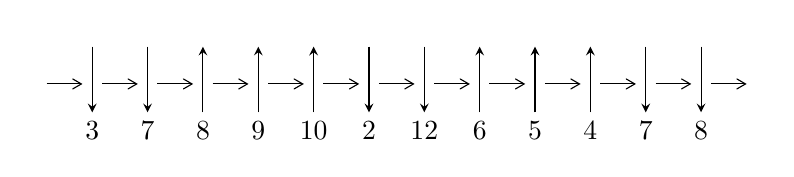
\begin{tikzpicture}[x=20pt, y=17pt]
	% nodes
	\node (C0) at (0, 0) {};
	\node (C1) at (1, 0) {};
	\node (C1U) at (1, +1) {};
	\node (C1D) at (1, -1) {3};

	\node (C2) at (2, 0) {};
	\node (C2U) at (2, +1) {};
	\node (C2D) at (2, -1) {7};

	\node (C3) at (3, 0) {};
	\node (C3U) at (3, +1) {};
	\node (C3D) at (3, -1) {8};

	\node (C4) at (4, 0) {};
	\node (C4U) at (4, +1) {};
	\node (C4D) at (4, -1) {9};

	\node (C5) at (5, 0) {};
	\node (C5U) at (5, +1) {};
	\node (C5D) at (5, -1) {10};

	\node (C6) at (6, 0) {};
	\node (C6U) at (6, +1) {};
	\node (C6D) at (6, -1) {2};

	\node (C7) at (7, 0) {};
	\node (C7U) at (7, +1) {};
	\node (C7D) at (7, -1) {12};

	\node (C8) at (8, 0) {};
	\node (C8U) at (8, +1) {};
	\node (C8D) at (8, -1) {6};

	\node (C9) at (9, 0) {};
	\node (C9U) at (9, +1) {};
	\node (C9D) at (9, -1) {5};

	\node (C10) at (10, 0) {};
	\node (C10U) at (10, +1) {};
	\node (C10D) at (10, -1) {4};

	\node (C11) at (11, 0) {};
	\node (C11U) at (11, +1) {};
	\node (C11D) at (11, -1) {7};

	\node (C12) at (12, 0) {};
	\node (C12U) at (12, +1) {};
	\node (C12D) at (12, -1) {8};
	\node (C13) at (13, 0) {};

	% arrows
	\draw[->,>={angle 60}]
	(C0) edge (C1) (C1) edge (C2) (C2) edge (C3) (C3) edge (C4) (C4) edge (C5) (C5) edge (C6) (C6) edge (C7) (C7) edge (C8) (C8) edge (C9) (C9) edge (C10) (C10) edge (C11) (C11) edge (C12) (C12) edge (C13) ;	\draw[->,>=stealth]
	(C1U) edge (C1D) (C2U) edge (C2D) (C3D) edge (C3U) (C4D) edge (C4U) (C5D) edge (C5U) (C6U) edge (C6D) (C7U) edge (C7D) (C8D) edge (C8U) (C9D) edge (C9U) (C10D) edge (C10U) (C11U) edge (C11D) (C12U) edge (C12D) ;
	\end{tikzpicture} \\
\hhline{~~} \\& 
\textbf{Solving Sequence} \\ \cline{2-2} 
 &
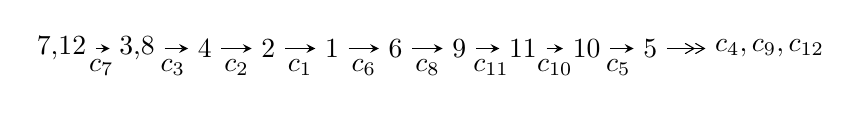
\begin{tikzpicture}[x=23pt, y=7pt]
	% node
	\node (A0) at (-1/8, 0) {7,12};
	\node (A1) at (17/16, 0) {3,8};
	\node (A2) at (17/8, 0) {4};
	\node (A3) at (25/8, 0) {2};
	\node (A4) at (33/8, 0) {1};
	\node (A5) at (41/8, 0) {6};
	\node (A6) at (49/8, 0) {9};
	\node (A7) at (57/8, 0) {11};
	\node (A8) at (65/8, 0) {10};
	\node (A9) at (73/8, 0) {5};
	\node (C1) at (1/2, -1) {$c_{7}$};
	\node (C2) at (13/8, -1) {$c_{3}$};
	\node (C3) at (21/8, -1) {$c_{2}$};
	\node (C4) at (29/8, -1) {$c_{1}$};
	\node (C5) at (37/8, -1) {$c_{6}$};
	\node (C6) at (45/8, -1) {$c_{8}$};
	\node (C7) at (53/8, -1) {$c_{11}$};
	\node (C8) at (61/8, -1) {$c_{10}$};
	\node (C9) at (69/8, -1) {$c_{5}$};
	\node (A10) at (11, 0) {$c_{4},c_{9},c_{12}$};

	% edge
	\draw[->,>=stealth]	
	(A0) edge (A1) (A1) edge (A2) (A2) edge (A3) (A3) edge (A4) (A4) edge (A5) (A5) edge (A6) (A6) edge (A7) (A7) edge (A8) (A8) edge (A9) ;
	\draw[->>,>={angle 60}]	
	(A9) edge (A10);
\end{tikzpicture} \\ 

\end{tabular} \\

\footnotetext{
The image of knot diagram is generated by the software ``\textbf{Draw programme}" developed by Andrew Bartholomew(\url{http://www.layer8.co.uk/maths/draw/index.htm\#Running-draw}), where we modified some parts for our purpose(\url{https://github.com/CATsTAILs/LinksPainter}).
}\phantom \\ \newline 
\centering \textbf{Ideals for irreducible components\footnotemark of $X_{\text{par}}$} 
 
\begin{align*}
I^u_{1}&=\langle 
b- u,\;u^{23}- u^{22}+\cdots+16 a+1,\;u^{25}- u^{24}+\cdots+3 u^2-1\rangle \\
I^u_{2}&=\langle 
-36334607050217 u^{29}+39477995355924 u^{28}+\cdots+2200950009156001 b-1119770521665287,\\
\phantom{I^u_{2}}&\phantom{= \langle  }- u^{29}+u^{28}+\cdots+7 a-6,\;u^{30}- u^{29}+\cdots+6 u+7\rangle \\
I^u_{3}&=\langle 
b+1,\;a^4+4 a^3+9 a^2+10 a+7,\;u-1\rangle \\
I^u_{4}&=\langle 
b-1,\;a^4-4 a^3+7 a^2-6 a+1,\;u+1\rangle \\
I^u_{5}&=\langle 
b+1,\;a+1,\;u-1\rangle \\
\\
\end{align*}
\raggedright * 5 irreducible components of $\dim_{\mathbb{C}}=0$, with total 64 representations.\\
\footnotetext{All coefficients of polynomials are rational numbers. But the coefficients are sometimes approximated in decimal forms when there is not enough margin.}
\newpage
\renewcommand{\arraystretch}{1}
\centering \section*{I. $I^u_{1}= \langle b- u,\;u^{23}- u^{22}+\cdots+16 a+1,\;u^{25}- u^{24}+\cdots+3 u^2-1 \rangle$}
\flushleft \textbf{(i) Arc colorings}\\
\begin{tabular}{m{7pt} m{180pt} m{7pt} m{180pt} }
\flushright $a_{7}=$&$\begin{pmatrix}1\\0\end{pmatrix}$ \\
\flushright $a_{12}=$&$\begin{pmatrix}0\\u\end{pmatrix}$ \\
\flushright $a_{3}=$&$\begin{pmatrix}-\frac{1}{16} u^{23}+\frac{1}{16} u^{22}+\cdots-2 u-\frac{1}{16}\\u\end{pmatrix}$ \\
\flushright $a_{8}=$&$\begin{pmatrix}1\\u^2\end{pmatrix}$ \\
\flushright $a_{4}=$&$\begin{pmatrix}- u\\\frac{1}{16} u^{23}-\frac{1}{16} u^{22}+\cdots+u+\frac{1}{16}\end{pmatrix}$ \\
\flushright $a_{2}=$&$\begin{pmatrix}-\frac{1}{16} u^{23}+\frac{1}{16} u^{22}+\cdots- u-\frac{1}{16}\\u\end{pmatrix}$ \\
\flushright $a_{1}=$&$\begin{pmatrix}- u\\- u^3+u\end{pmatrix}$ \\
\flushright $a_{6}=$&$\begin{pmatrix}\frac{1}{16} u^{24}-\frac{1}{16} u^{23}+\cdots+\frac{1}{16} u+1\\- u^2\end{pmatrix}$ \\
\flushright $a_{9}=$&$\begin{pmatrix}\frac{9}{16} u^{24}-\frac{5}{8} u^{23}+\cdots+\frac{11}{16} u+\frac{15}{16}\\-\frac{1}{16} u^{24}+\frac{1}{16} u^{23}+\cdots+u^2-\frac{1}{16} u\end{pmatrix}$ \\
\flushright $a_{11}=$&$\begin{pmatrix}u\\u\end{pmatrix}$ \\
\flushright $a_{10}=$&$\begin{pmatrix}-\frac{1}{16} u^{23}+\frac{1}{16} u^{22}+\cdots+u-\frac{1}{16}\\-0.0625000 u^{24}+0.500000 u^{23}+\cdots+0.937500 u+0.562500\end{pmatrix}$ \\
\flushright $a_{5}=$&$\begin{pmatrix}1.18750 u^{24}-1.81250 u^{23}+\cdots+0.812500 u+0.625000\\-0.625000 u^{24}+1.43750 u^{23}+\cdots+0.625000 u+1.18750\end{pmatrix}$\\&\end{tabular}
\flushleft \textbf{(ii) Obstruction class $= -1$}\\~\\
\flushleft \textbf{(iii) Cusp Shapes $= \frac{9}{4} u^{24}-\frac{15}{8} u^{23}+\cdots+u-\frac{19}{8}$}\\~\\
\newpage\renewcommand{\arraystretch}{1}
\flushleft \textbf{(iv) u-Polynomials at the component}\newline \\
\begin{tabular}{m{50pt}|m{274pt}}
Crossings & \hspace{64pt}u-Polynomials at each crossing \\
\hline $$\begin{aligned}c_{1}\end{aligned}$$&$\begin{aligned}
&u^{25}+7 u^{24}+\cdots+6 u+1
\end{aligned}$\\
\hline $$\begin{aligned}c_{2},c_{6},c_{7}\\c_{11},c_{12}\end{aligned}$$&$\begin{aligned}
&u^{25}- u^{24}+\cdots+3 u^2-1
\end{aligned}$\\
\hline $$\begin{aligned}c_{3}\end{aligned}$$&$\begin{aligned}
&u^{25}+3 u^{24}+\cdots-688 u-178
\end{aligned}$\\
\hline $$\begin{aligned}c_{4},c_{5},c_{9}\end{aligned}$$&$\begin{aligned}
&u^{25}-3 u^{24}+\cdots-5 u^2-2
\end{aligned}$\\
\hline $$\begin{aligned}c_{8},c_{10}\end{aligned}$$&$\begin{aligned}
&u^{25}+9 u^{24}+\cdots+92 u+14
\end{aligned}$\\
\hline
\end{tabular}\\~\\
\newpage\renewcommand{\arraystretch}{1}
\flushleft \textbf{(v) Riley Polynomials at the component}\newline \\
\begin{tabular}{m{50pt}|m{274pt}}
Crossings & \hspace{64pt}Riley Polynomials at each crossing \\
\hline $$\begin{aligned}c_{1}\end{aligned}$$&$\begin{aligned}
&y^{25}+33 y^{24}+\cdots+2 y-1
\end{aligned}$\\
\hline $$\begin{aligned}c_{2},c_{6},c_{7}\\c_{11},c_{12}\end{aligned}$$&$\begin{aligned}
&y^{25}-7 y^{24}+\cdots+6 y-1
\end{aligned}$\\
\hline $$\begin{aligned}c_{3}\end{aligned}$$&$\begin{aligned}
&y^{25}-9 y^{24}+\cdots-428404 y-31684
\end{aligned}$\\
\hline $$\begin{aligned}c_{4},c_{5},c_{9}\end{aligned}$$&$\begin{aligned}
&y^{25}-21 y^{24}+\cdots-20 y-4
\end{aligned}$\\
\hline $$\begin{aligned}c_{8},c_{10}\end{aligned}$$&$\begin{aligned}
&y^{25}+15 y^{24}+\cdots-244 y-196
\end{aligned}$\\
\hline
\end{tabular}\\~\\
\newpage\flushleft \textbf{(vi) Complex Volumes and Cusp Shapes}
$$\begin{array}{c|c|c}  
\text{Solutions to }I^u_{1}& \I (\text{vol} + \sqrt{-1}CS) & \text{Cusp shape}\\
 \hline 
\begin{aligned}
u &= -0.785518 + 0.372640 I \\
a &= \phantom{-}0.62353 - 2.12777 I \\
b &= -0.785518 + 0.372640 I\end{aligned}
 & -2.17521 + 5.68827 I & -0.75349 - 8.49425 I \\ \hline\begin{aligned}
u &= -0.785518 - 0.372640 I \\
a &= \phantom{-}0.62353 + 2.12777 I \\
b &= -0.785518 - 0.372640 I\end{aligned}
 & -2.17521 - 5.68827 I & -0.75349 + 8.49425 I \\ \hline\begin{aligned}
u &= \phantom{-}0.755648 + 0.329653 I \\
a &= -0.90101 - 2.06111 I \\
b &= \phantom{-}0.755648 + 0.329653 I\end{aligned}
 & -6.02340 - 1.36429 I & -4.30078 + 5.12755 I \\ \hline\begin{aligned}
u &= \phantom{-}0.755648 - 0.329653 I \\
a &= -0.90101 + 2.06111 I \\
b &= \phantom{-}0.755648 - 0.329653 I\end{aligned}
 & -6.02340 + 1.36429 I & -4.30078 - 5.12755 I \\ \hline\begin{aligned}
u &= -0.845914 + 0.820525 I \\
a &= -0.231288 - 1.378290 I \\
b &= -0.845914 + 0.820525 I\end{aligned}
 & \phantom{-}1.53021 + 1.97230 I & -1.25071 - 1.01903 I \\ \hline\begin{aligned}
u &= -0.845914 - 0.820525 I \\
a &= -0.231288 + 1.378290 I \\
b &= -0.845914 - 0.820525 I\end{aligned}
 & \phantom{-}1.53021 - 1.97230 I & -1.25071 + 1.01903 I \\ \hline\begin{aligned}
u &= \phantom{-}0.265507 + 0.770529 I \\
a &= -0.071679 - 1.030960 I \\
b &= \phantom{-}0.265507 + 0.770529 I\end{aligned}
 & \phantom{-}4.72198 - 3.16963 I & \phantom{-}6.44572 + 4.63465 I \\ \hline\begin{aligned}
u &= \phantom{-}0.265507 - 0.770529 I \\
a &= -0.071679 + 1.030960 I \\
b &= \phantom{-}0.265507 - 0.770529 I\end{aligned}
 & \phantom{-}4.72198 + 3.16963 I & \phantom{-}6.44572 - 4.63465 I \\ \hline\begin{aligned}
u &= -0.730832 + 0.286998 I \\
a &= \phantom{-}1.17630 - 1.94700 I \\
b &= -0.730832 + 0.286998 I\end{aligned}
 & -2.02761 - 2.93831 I & \phantom{-}0.12922 - 1.80135 I \\ \hline\begin{aligned}
u &= -0.730832 - 0.286998 I \\
a &= \phantom{-}1.17630 + 1.94700 I \\
b &= -0.730832 - 0.286998 I\end{aligned}
 & -2.02761 + 2.93831 I & \phantom{-}0.12922 + 1.80135 I\\
 \hline 
 \end{array}$$\newpage$$\begin{array}{c|c|c}  
\text{Solutions to }I^u_{1}& \I (\text{vol} + \sqrt{-1}CS) & \text{Cusp shape}\\
 \hline 
\begin{aligned}
u &= \phantom{-}0.964582 + 0.777415 I \\
a &= \phantom{-}0.38162 - 1.45780 I \\
b &= \phantom{-}0.964582 + 0.777415 I\end{aligned}
 & \phantom{-}3.01562 - 5.74190 I & \phantom{-}0.65811 + 6.60844 I \\ \hline\begin{aligned}
u &= \phantom{-}0.964582 - 0.777415 I \\
a &= \phantom{-}0.38162 + 1.45780 I \\
b &= \phantom{-}0.964582 - 0.777415 I\end{aligned}
 & \phantom{-}3.01562 + 5.74190 I & \phantom{-}0.65811 - 6.60844 I \\ \hline\begin{aligned}
u &= \phantom{-}0.834411 + 0.917128 I \\
a &= \phantom{-}0.245471 - 1.273980 I \\
b &= \phantom{-}0.834411 + 0.917128 I\end{aligned}
 & \phantom{-}6.70653 + 1.49728 I & \phantom{-}3.61002 - 0.12989 I \\ \hline\begin{aligned}
u &= \phantom{-}0.834411 - 0.917128 I \\
a &= \phantom{-}0.245471 + 1.273980 I \\
b &= \phantom{-}0.834411 - 0.917128 I\end{aligned}
 & \phantom{-}6.70653 - 1.49728 I & \phantom{-}3.61002 + 0.12989 I \\ \hline\begin{aligned}
u &= \phantom{-}1.075630 + 0.727569 I \\
a &= \phantom{-}0.57040 - 1.51015 I \\
b &= \phantom{-}1.075630 + 0.727569 I\end{aligned}
 & \phantom{-}2.19442 - 6.05278 I & -0.77143 + 3.74618 I \\ \hline\begin{aligned}
u &= \phantom{-}1.075630 - 0.727569 I \\
a &= \phantom{-}0.57040 + 1.51015 I \\
b &= \phantom{-}1.075630 - 0.727569 I\end{aligned}
 & \phantom{-}2.19442 + 6.05278 I & -0.77143 - 3.74618 I \\ \hline\begin{aligned}
u &= -1.129150 + 0.745345 I \\
a &= -0.64410 - 1.44902 I \\
b &= -1.129150 + 0.745345 I\end{aligned}
 & -0.44383 + 10.34840 I & -3.77176 - 7.45516 I \\ \hline\begin{aligned}
u &= -1.129150 - 0.745345 I \\
a &= -0.64410 + 1.44902 I \\
b &= -1.129150 - 0.745345 I\end{aligned}
 & -0.44383 - 10.34840 I & -3.77176 + 7.45516 I \\ \hline\begin{aligned}
u &= -1.040970 + 0.866286 I \\
a &= -0.469635 - 1.328000 I \\
b &= -1.040970 + 0.866286 I\end{aligned}
 & \phantom{-}9.76977 + 6.71873 I & \phantom{-}4.67666 - 4.93521 I \\ \hline\begin{aligned}
u &= -1.040970 - 0.866286 I \\
a &= -0.469635 + 1.328000 I \\
b &= -1.040970 - 0.866286 I\end{aligned}
 & \phantom{-}9.76977 - 6.71873 I & \phantom{-}4.67666 + 4.93521 I\\
 \hline 
 \end{array}$$\newpage$$\begin{array}{c|c|c}  
\text{Solutions to }I^u_{1}& \I (\text{vol} + \sqrt{-1}CS) & \text{Cusp shape}\\
 \hline 
\begin{aligned}
u &= \phantom{-}1.156880 + 0.765655 I \\
a &= \phantom{-}0.66857 - 1.39962 I \\
b &= \phantom{-}1.156880 + 0.765655 I\end{aligned}
 & \phantom{-}4.4401 - 14.5092 I & \phantom{-}0.55817 + 8.79115 I \\ \hline\begin{aligned}
u &= \phantom{-}1.156880 - 0.765655 I \\
a &= \phantom{-}0.66857 + 1.39962 I \\
b &= \phantom{-}1.156880 - 0.765655 I\end{aligned}
 & \phantom{-}4.4401 + 14.5092 I & \phantom{-}0.55817 - 8.79115 I \\ \hline\begin{aligned}
u &= -0.260838 + 0.456783 I \\
a &= \phantom{-}0.277904 - 0.859001 I \\
b &= -0.260838 + 0.456783 I\end{aligned}
 & \phantom{-}0.037229 + 0.975136 I & \phantom{-}0.76804 - 7.07893 I \\ \hline\begin{aligned}
u &= -0.260838 - 0.456783 I \\
a &= \phantom{-}0.277904 + 0.859001 I \\
b &= -0.260838 - 0.456783 I\end{aligned}
 & \phantom{-}0.037229 - 0.975136 I & \phantom{-}0.76804 + 7.07893 I \\ \hline\begin{aligned}
u &= \phantom{-}0.481143\phantom{ +0.000000I} \\
a &= -1.25216\phantom{ +0.000000I} \\
b &= \phantom{-}0.481143\phantom{ +0.000000I}\end{aligned}
 & \phantom{-}2.56662\phantom{ +0.000000I} & \phantom{-}2.00450\phantom{ +0.000000I}\\
 \hline 
 \end{array}$$\newpage\newpage\renewcommand{\arraystretch}{1}
\centering \section*{II. $I^u_{2}= \langle -3.63\times10^{13} u^{29}+3.95\times10^{13} u^{28}+\cdots+2.20\times10^{15} b-1.12\times10^{15},\;- u^{29}+u^{28}+\cdots+7 a-6,\;u^{30}- u^{29}+\cdots+6 u+7 \rangle$}
\flushleft \textbf{(i) Arc colorings}\\
\begin{tabular}{m{7pt} m{180pt} m{7pt} m{180pt} }
\flushright $a_{7}=$&$\begin{pmatrix}1\\0\end{pmatrix}$ \\
\flushright $a_{12}=$&$\begin{pmatrix}0\\u\end{pmatrix}$ \\
\flushright $a_{3}=$&$\begin{pmatrix}\frac{1}{7} u^{29}-\frac{1}{7} u^{28}+\cdots-\frac{76}{7} u+\frac{6}{7}\\0.0165086 u^{29}-0.0179368 u^{28}+\cdots-3.56720 u+0.508767\end{pmatrix}$ \\
\flushright $a_{8}=$&$\begin{pmatrix}1\\u^2\end{pmatrix}$ \\
\flushright $a_{4}=$&$\begin{pmatrix}0.159366 u^{29}-0.160794 u^{28}+\cdots-13.4243 u+1.36591\\0.139320 u^{29}-0.0522821 u^{28}+\cdots-3.67419 u+0.518764\end{pmatrix}$ \\
\flushright $a_{2}=$&$\begin{pmatrix}0.159366 u^{29}-0.160794 u^{28}+\cdots-14.4243 u+1.36591\\0.0165086 u^{29}-0.0179368 u^{28}+\cdots-3.56720 u+0.508767\end{pmatrix}$ \\
\flushright $a_{1}=$&$\begin{pmatrix}- u\\- u^3+u\end{pmatrix}$ \\
\flushright $a_{6}=$&$\begin{pmatrix}-0.0741092 u^{29}+0.213429 u^{28}+\cdots+2.77558 u-4.11884\\-0.00142820 u^{29}+0.124240 u^{28}+\cdots+0.409715 u-1.11556\end{pmatrix}$ \\
\flushright $a_{9}=$&$\begin{pmatrix}-0.156177 u^{29}+0.104902 u^{28}+\cdots+1.37289 u-3.42762\\-0.173390 u^{29}+0.0449879 u^{28}+\cdots+0.143610 u-0.680215\end{pmatrix}$ \\
\flushright $a_{11}=$&$\begin{pmatrix}u\\u\end{pmatrix}$ \\
\flushright $a_{10}=$&$\begin{pmatrix}0.0971736 u^{29}-0.270564 u^{28}+\cdots-12.6008 u+0.726652\\-0.0512747 u^{29}-0.0842981 u^{28}+\cdots-2.49055 u+1.09324\end{pmatrix}$ \\
\flushright $a_{5}=$&$\begin{pmatrix}-0.167585 u^{29}-0.278986 u^{28}+\cdots-14.6020 u-3.43422\\-0.446571 u^{29}-0.0855200 u^{28}+\cdots-2.42870 u+1.17310\end{pmatrix}$\\&\end{tabular}
\flushleft \textbf{(ii) Obstruction class $= -1$}\\~\\
\flushleft \textbf{(iii) Cusp Shapes $= -\frac{2576715548071340}{2200950009156001} u^{29}-\frac{754152713873936}{2200950009156001} u^{28}+\cdots+\frac{5415273681221840}{2200950009156001} u+\frac{25651780906655686}{2200950009156001}$}\\~\\
\newpage\renewcommand{\arraystretch}{1}
\flushleft \textbf{(iv) u-Polynomials at the component}\newline \\
\begin{tabular}{m{50pt}|m{274pt}}
Crossings & \hspace{64pt}u-Polynomials at each crossing \\
\hline $$\begin{aligned}c_{1}\end{aligned}$$&$\begin{aligned}
&u^{30}+13 u^{29}+\cdots+1100 u+49
\end{aligned}$\\
\hline $$\begin{aligned}c_{2},c_{6},c_{7}\\c_{11},c_{12}\end{aligned}$$&$\begin{aligned}
&u^{30}- u^{29}+\cdots+6 u+7
\end{aligned}$\\
\hline $$\begin{aligned}c_{3}\end{aligned}$$&$\begin{aligned}
&(u^{15}- u^{14}+\cdots-2 u-1)^{2}
\end{aligned}$\\
\hline $$\begin{aligned}c_{4},c_{5},c_{9}\end{aligned}$$&$\begin{aligned}
&(u^{15}+u^{14}+\cdots-2 u-1)^{2}
\end{aligned}$\\
\hline $$\begin{aligned}c_{8},c_{10}\end{aligned}$$&$\begin{aligned}
&(u^{15}-3 u^{14}+\cdots+4 u^2-1)^{2}
\end{aligned}$\\
\hline
\end{tabular}\\~\\
\newpage\renewcommand{\arraystretch}{1}
\flushleft \textbf{(v) Riley Polynomials at the component}\newline \\
\begin{tabular}{m{50pt}|m{274pt}}
Crossings & \hspace{64pt}Riley Polynomials at each crossing \\
\hline $$\begin{aligned}c_{1}\end{aligned}$$&$\begin{aligned}
&y^{30}+7 y^{29}+\cdots-441680 y+2401
\end{aligned}$\\
\hline $$\begin{aligned}c_{2},c_{6},c_{7}\\c_{11},c_{12}\end{aligned}$$&$\begin{aligned}
&y^{30}-13 y^{29}+\cdots-1100 y+49
\end{aligned}$\\
\hline $$\begin{aligned}c_{3}\end{aligned}$$&$\begin{aligned}
&(y^{15}-17 y^{14}+\cdots+8 y-1)^{2}
\end{aligned}$\\
\hline $$\begin{aligned}c_{4},c_{5},c_{9}\end{aligned}$$&$\begin{aligned}
&(y^{15}-13 y^{14}+\cdots+8 y-1)^{2}
\end{aligned}$\\
\hline $$\begin{aligned}c_{8},c_{10}\end{aligned}$$&$\begin{aligned}
&(y^{15}+7 y^{14}+\cdots+8 y-1)^{2}
\end{aligned}$\\
\hline
\end{tabular}\\~\\
\newpage\flushleft \textbf{(vi) Complex Volumes and Cusp Shapes}
$$\begin{array}{c|c|c}  
\text{Solutions to }I^u_{2}& \I (\text{vol} + \sqrt{-1}CS) & \text{Cusp shape}\\
 \hline 
\begin{aligned}
u &= \phantom{-}0.933632 + 0.405000 I \\
a &= -0.901456 + 0.391043 I \\
b &= -1.243160 + 0.162791 I\end{aligned}
 & -1.99092 + 1.64925 I & -2.39367 - 0.16522 I \\ \hline\begin{aligned}
u &= \phantom{-}0.933632 - 0.405000 I \\
a &= -0.901456 - 0.391043 I \\
b &= -1.243160 - 0.162791 I\end{aligned}
 & -1.99092 - 1.64925 I & -2.39367 + 0.16522 I \\ \hline\begin{aligned}
u &= \phantom{-}0.666225 + 0.833796 I \\
a &= -0.584884 + 0.731996 I \\
b &= \phantom{-}0.815806 - 0.779519 I\end{aligned}
 & \phantom{-}3.47397 + 0.15908 I & \phantom{-}1.79403 + 0.85194 I \\ \hline\begin{aligned}
u &= \phantom{-}0.666225 - 0.833796 I \\
a &= -0.584884 - 0.731996 I \\
b &= \phantom{-}0.815806 + 0.779519 I\end{aligned}
 & \phantom{-}3.47397 - 0.15908 I & \phantom{-}1.79403 - 0.85194 I \\ \hline\begin{aligned}
u &= -0.786352 + 0.445678 I \\
a &= \phantom{-}0.962512 + 0.545520 I \\
b &= \phantom{-}1.273190 + 0.075844 I\end{aligned}
 & -5.46412 + 1.81248 I & -5.85619 - 4.33913 I \\ \hline\begin{aligned}
u &= -0.786352 - 0.445678 I \\
a &= \phantom{-}0.962512 - 0.545520 I \\
b &= \phantom{-}1.273190 - 0.075844 I\end{aligned}
 & -5.46412 - 1.81248 I & -5.85619 + 4.33913 I \\ \hline\begin{aligned}
u &= \phantom{-}1.10731\phantom{ +0.000000I} \\
a &= -0.903090\phantom{ +0.000000I} \\
b &= -0.270107\phantom{ +0.000000I}\end{aligned}
 & \phantom{-}2.23561\phantom{ +0.000000I} & \phantom{-}5.03940\phantom{ +0.000000I} \\ \hline\begin{aligned}
u &= -0.582390 + 0.944453 I \\
a &= \phantom{-}0.473038 + 0.767119 I \\
b &= -0.944169 - 0.806161 I\end{aligned}
 & \phantom{-}1.23287 - 4.11725 I & -1.40312 + 3.71929 I \\ \hline\begin{aligned}
u &= -0.582390 - 0.944453 I \\
a &= \phantom{-}0.473038 - 0.767119 I \\
b &= -0.944169 + 0.806161 I\end{aligned}
 & \phantom{-}1.23287 + 4.11725 I & -1.40312 - 3.71929 I \\ \hline\begin{aligned}
u &= \phantom{-}0.815806 + 0.779519 I \\
a &= -0.640758 + 0.612257 I \\
b &= \phantom{-}0.666225 - 0.833796 I\end{aligned}
 & \phantom{-}3.47397 - 0.15908 I & \phantom{-}1.79403 - 0.85194 I\\
 \hline 
 \end{array}$$\newpage$$\begin{array}{c|c|c}  
\text{Solutions to }I^u_{2}& \I (\text{vol} + \sqrt{-1}CS) & \text{Cusp shape}\\
 \hline 
\begin{aligned}
u &= \phantom{-}0.815806 - 0.779519 I \\
a &= -0.640758 - 0.612257 I \\
b &= \phantom{-}0.666225 + 0.833796 I\end{aligned}
 & \phantom{-}3.47397 + 0.15908 I & \phantom{-}1.79403 + 0.85194 I \\ \hline\begin{aligned}
u &= \phantom{-}0.689418 + 0.518899 I \\
a &= -0.925949 + 0.696926 I \\
b &= -1.305660 + 0.019757 I\end{aligned}
 & -1.10658 - 5.45324 I & -0.00468 + 6.35130 I \\ \hline\begin{aligned}
u &= \phantom{-}0.689418 - 0.518899 I \\
a &= -0.925949 - 0.696926 I \\
b &= -1.305660 - 0.019757 I\end{aligned}
 & -1.10658 + 5.45324 I & -0.00468 - 6.35130 I \\ \hline\begin{aligned}
u &= -1.13884\phantom{ +0.000000I} \\
a &= \phantom{-}0.878083\phantom{ +0.000000I} \\
b &= \phantom{-}0.734573\phantom{ +0.000000I}\end{aligned}
 & -2.69194\phantom{ +0.000000I} & \phantom{-}4.62820\phantom{ +0.000000I} \\ \hline\begin{aligned}
u &= \phantom{-}0.583255 + 1.014300 I \\
a &= -0.426049 + 0.740911 I \\
b &= \phantom{-}0.987724 - 0.853962 I\end{aligned}
 & \phantom{-}6.22908 + 8.01682 I & \phantom{-}3.04132 - 4.89679 I \\ \hline\begin{aligned}
u &= \phantom{-}0.583255 - 1.014300 I \\
a &= -0.426049 - 0.740911 I \\
b &= \phantom{-}0.987724 + 0.853962 I\end{aligned}
 & \phantom{-}6.22908 - 8.01682 I & \phantom{-}3.04132 + 4.89679 I \\ \hline\begin{aligned}
u &= -0.944169 + 0.806161 I \\
a &= \phantom{-}0.612560 + 0.523023 I \\
b &= -0.582390 - 0.944453 I\end{aligned}
 & \phantom{-}1.23287 + 4.11725 I & -1.40312 - 3.71929 I \\ \hline\begin{aligned}
u &= -0.944169 - 0.806161 I \\
a &= \phantom{-}0.612560 - 0.523023 I \\
b &= -0.582390 + 0.944453 I\end{aligned}
 & \phantom{-}1.23287 - 4.11725 I & -1.40312 + 3.71929 I \\ \hline\begin{aligned}
u &= -1.243160 + 0.162791 I \\
a &= \phantom{-}0.790842 + 0.103561 I \\
b &= \phantom{-}0.933632 + 0.405000 I\end{aligned}
 & -1.99092 + 1.64925 I & -2.39367 - 0.16522 I \\ \hline\begin{aligned}
u &= -1.243160 - 0.162791 I \\
a &= \phantom{-}0.790842 - 0.103561 I \\
b &= \phantom{-}0.933632 - 0.405000 I\end{aligned}
 & -1.99092 - 1.64925 I & -2.39367 + 0.16522 I\\
 \hline 
 \end{array}$$\newpage$$\begin{array}{c|c|c}  
\text{Solutions to }I^u_{2}& \I (\text{vol} + \sqrt{-1}CS) & \text{Cusp shape}\\
 \hline 
\begin{aligned}
u &= -0.803987 + 0.969115 I \\
a &= \phantom{-}0.507062 + 0.611206 I \\
b &= -0.803987 - 0.969115 I\end{aligned}
 & \phantom{-}10.5121\phantom{ +0.000000I} & \phantom{-}5.97706 + 0. I\phantom{ +0.000000I} \\ \hline\begin{aligned}
u &= -0.803987 - 0.969115 I \\
a &= \phantom{-}0.507062 - 0.611206 I \\
b &= -0.803987 + 0.969115 I\end{aligned}
 & \phantom{-}10.5121\phantom{ +0.000000I} & \phantom{-}5.97706 + 0. I\phantom{ +0.000000I} \\ \hline\begin{aligned}
u &= \phantom{-}0.734573\phantom{ +0.000000I} \\
a &= -1.36134\phantom{ +0.000000I} \\
b &= -1.13884\phantom{ +0.000000I}\end{aligned}
 & -2.69194\phantom{ +0.000000I} & \phantom{-}4.62820\phantom{ +0.000000I} \\ \hline\begin{aligned}
u &= \phantom{-}1.273190 + 0.075844 I \\
a &= -0.782653 + 0.046623 I \\
b &= -0.786352 + 0.445678 I\end{aligned}
 & -5.46412 + 1.81248 I & -5.85619 - 4.33913 I \\ \hline\begin{aligned}
u &= \phantom{-}1.273190 - 0.075844 I \\
a &= -0.782653 - 0.046623 I \\
b &= -0.786352 - 0.445678 I\end{aligned}
 & -5.46412 - 1.81248 I & -5.85619 + 4.33913 I \\ \hline\begin{aligned}
u &= \phantom{-}0.987724 + 0.853962 I \\
a &= -0.579361 + 0.500902 I \\
b &= \phantom{-}0.583255 - 1.014300 I\end{aligned}
 & \phantom{-}6.22908 - 8.01682 I & \phantom{-}3.04132 + 4.89679 I \\ \hline\begin{aligned}
u &= \phantom{-}0.987724 - 0.853962 I \\
a &= -0.579361 - 0.500902 I \\
b &= \phantom{-}0.583255 + 1.014300 I\end{aligned}
 & \phantom{-}6.22908 + 8.01682 I & \phantom{-}3.04132 - 4.89679 I \\ \hline\begin{aligned}
u &= -1.305660 + 0.019757 I \\
a &= \phantom{-}0.765721 + 0.011587 I \\
b &= \phantom{-}0.689418 + 0.518899 I\end{aligned}
 & -1.10658 - 5.45324 I & -0.00468 + 6.35130 I \\ \hline\begin{aligned}
u &= -1.305660 - 0.019757 I \\
a &= \phantom{-}0.765721 - 0.011587 I \\
b &= \phantom{-}0.689418 - 0.518899 I\end{aligned}
 & -1.10658 + 5.45324 I & -0.00468 - 6.35130 I \\ \hline\begin{aligned}
u &= -0.270107\phantom{ +0.000000I} \\
a &= \phantom{-}3.70223\phantom{ +0.000000I} \\
b &= \phantom{-}1.10731\phantom{ +0.000000I}\end{aligned}
 & \phantom{-}2.23561\phantom{ +0.000000I} & \phantom{-}5.03940\phantom{ +0.000000I}\\
 \hline 
 \end{array}$$\newpage\newpage\renewcommand{\arraystretch}{1}
\centering \section*{III. $I^u_{3}= \langle b+1,\;a^4+4 a^3+9 a^2+10 a+7,\;u-1 \rangle$}
\flushleft \textbf{(i) Arc colorings}\\
\begin{tabular}{m{7pt} m{180pt} m{7pt} m{180pt} }
\flushright $a_{7}=$&$\begin{pmatrix}1\\0\end{pmatrix}$ \\
\flushright $a_{12}=$&$\begin{pmatrix}0\\1\end{pmatrix}$ \\
\flushright $a_{3}=$&$\begin{pmatrix}a\\-1\end{pmatrix}$ \\
\flushright $a_{8}=$&$\begin{pmatrix}1\\1\end{pmatrix}$ \\
\flushright $a_{4}=$&$\begin{pmatrix}-1\\- a-2\end{pmatrix}$ \\
\flushright $a_{2}=$&$\begin{pmatrix}a-1\\-1\end{pmatrix}$ \\
\flushright $a_{1}=$&$\begin{pmatrix}-1\\0\end{pmatrix}$ \\
\flushright $a_{6}=$&$\begin{pmatrix}a\\-1\end{pmatrix}$ \\
\flushright $a_{9}=$&$\begin{pmatrix}a^2+a+1\\- a\end{pmatrix}$ \\
\flushright $a_{11}=$&$\begin{pmatrix}1\\1\end{pmatrix}$ \\
\flushright $a_{10}=$&$\begin{pmatrix}a+2\\a^2+3 a+3\end{pmatrix}$ \\
\flushright $a_{5}=$&$\begin{pmatrix}a^3+a^2+a-3\\- a^3-5 a^2-9 a-9\end{pmatrix}$\\&\end{tabular}
\flushleft \textbf{(ii) Obstruction class $= 1$}\\~\\
\flushleft \textbf{(iii) Cusp Shapes $= -4 a^2-8 a-16$}\\~\\
\newpage\renewcommand{\arraystretch}{1}
\flushleft \textbf{(iv) u-Polynomials at the component}\newline \\
\begin{tabular}{m{50pt}|m{274pt}}
Crossings & \hspace{64pt}u-Polynomials at each crossing \\
\hline $$\begin{aligned}c_{1},c_{2},c_{7}\end{aligned}$$&$\begin{aligned}
&(u-1)^4
\end{aligned}$\\
\hline $$\begin{aligned}c_{3},c_{8},c_{10}\end{aligned}$$&$\begin{aligned}
&u^4+3 u^2+3
\end{aligned}$\\
\hline $$\begin{aligned}c_{4},c_{5},c_{9}\end{aligned}$$&$\begin{aligned}
&u^4-3 u^2+3
\end{aligned}$\\
\hline $$\begin{aligned}c_{6},c_{11},c_{12}\end{aligned}$$&$\begin{aligned}
&(u+1)^4
\end{aligned}$\\
\hline
\end{tabular}\\~\\
\newpage\renewcommand{\arraystretch}{1}
\flushleft \textbf{(v) Riley Polynomials at the component}\newline \\
\begin{tabular}{m{50pt}|m{274pt}}
Crossings & \hspace{64pt}Riley Polynomials at each crossing \\
\hline $$\begin{aligned}c_{1},c_{2},c_{6}\\c_{7},c_{11},c_{12}\end{aligned}$$&$\begin{aligned}
&(y-1)^4
\end{aligned}$\\
\hline $$\begin{aligned}c_{3},c_{8},c_{10}\end{aligned}$$&$\begin{aligned}
&(y^2+3 y+3)^2
\end{aligned}$\\
\hline $$\begin{aligned}c_{4},c_{5},c_{9}\end{aligned}$$&$\begin{aligned}
&(y^2-3 y+3)^2
\end{aligned}$\\
\hline
\end{tabular}\\~\\
\newpage\flushleft \textbf{(vi) Complex Volumes and Cusp Shapes}
$$\begin{array}{c|c|c}  
\text{Solutions to }I^u_{3}& \I (\text{vol} + \sqrt{-1}CS) & \text{Cusp shape}\\
 \hline 
\begin{aligned}
u &= \phantom{-}1.00000\phantom{ +0.000000I} \\
a &= -0.65937 + 1.27123 I \\
b &= -1.00000\phantom{ +0.000000I}\end{aligned}
 & -3.28987 + 4.05977 I & -6.00000 - 3.46410 I \\ \hline\begin{aligned}
u &= \phantom{-}1.00000\phantom{ +0.000000I} \\
a &= -0.65937 - 1.27123 I \\
b &= -1.00000\phantom{ +0.000000I}\end{aligned}
 & -3.28987 - 4.05977 I & -6.00000 + 3.46410 I \\ \hline\begin{aligned}
u &= \phantom{-}1.00000\phantom{ +0.000000I} \\
a &= -1.34063 + 1.27123 I \\
b &= -1.00000\phantom{ +0.000000I}\end{aligned}
 & -3.28987 - 4.05977 I & -6.00000 + 3.46410 I \\ \hline\begin{aligned}
u &= \phantom{-}1.00000\phantom{ +0.000000I} \\
a &= -1.34063 - 1.27123 I \\
b &= -1.00000\phantom{ +0.000000I}\end{aligned}
 & -3.28987 + 4.05977 I & -6.00000 - 3.46410 I\\
 \hline 
 \end{array}$$\newpage\newpage\renewcommand{\arraystretch}{1}
\centering \section*{IV. $I^u_{4}= \langle b-1,\;a^4-4 a^3+7 a^2-6 a+1,\;u+1 \rangle$}
\flushleft \textbf{(i) Arc colorings}\\
\begin{tabular}{m{7pt} m{180pt} m{7pt} m{180pt} }
\flushright $a_{7}=$&$\begin{pmatrix}1\\0\end{pmatrix}$ \\
\flushright $a_{12}=$&$\begin{pmatrix}0\\-1\end{pmatrix}$ \\
\flushright $a_{3}=$&$\begin{pmatrix}a\\1\end{pmatrix}$ \\
\flushright $a_{8}=$&$\begin{pmatrix}1\\1\end{pmatrix}$ \\
\flushright $a_{4}=$&$\begin{pmatrix}1\\- a+2\end{pmatrix}$ \\
\flushright $a_{2}=$&$\begin{pmatrix}a+1\\1\end{pmatrix}$ \\
\flushright $a_{1}=$&$\begin{pmatrix}1\\0\end{pmatrix}$ \\
\flushright $a_{6}=$&$\begin{pmatrix}- a\\-1\end{pmatrix}$ \\
\flushright $a_{9}=$&$\begin{pmatrix}a^2- a+1\\a\end{pmatrix}$ \\
\flushright $a_{11}=$&$\begin{pmatrix}-1\\-1\end{pmatrix}$ \\
\flushright $a_{10}=$&$\begin{pmatrix}a-2\\- a^2+3 a-3\end{pmatrix}$ \\
\flushright $a_{5}=$&$\begin{pmatrix}- a^3+3 a^2-5 a+3\\- a^3+3 a^2-5 a+3\end{pmatrix}$\\&\end{tabular}
\flushleft \textbf{(ii) Obstruction class $= 1$}\\~\\
\flushleft \textbf{(iii) Cusp Shapes $= 4 a^2-8 a$}\\~\\
\newpage\renewcommand{\arraystretch}{1}
\flushleft \textbf{(iv) u-Polynomials at the component}\newline \\
\begin{tabular}{m{50pt}|m{274pt}}
Crossings & \hspace{64pt}u-Polynomials at each crossing \\
\hline $$\begin{aligned}c_{1},c_{6},c_{11}\\c_{12}\end{aligned}$$&$\begin{aligned}
&(u-1)^4
\end{aligned}$\\
\hline $$\begin{aligned}c_{2},c_{7}\end{aligned}$$&$\begin{aligned}
&(u+1)^4
\end{aligned}$\\
\hline $$\begin{aligned}c_{3},c_{8},c_{10}\end{aligned}$$&$\begin{aligned}
&u^4+u^2-1
\end{aligned}$\\
\hline $$\begin{aligned}c_{4},c_{5},c_{9}\end{aligned}$$&$\begin{aligned}
&u^4- u^2-1
\end{aligned}$\\
\hline
\end{tabular}\\~\\
\newpage\renewcommand{\arraystretch}{1}
\flushleft \textbf{(v) Riley Polynomials at the component}\newline \\
\begin{tabular}{m{50pt}|m{274pt}}
Crossings & \hspace{64pt}Riley Polynomials at each crossing \\
\hline $$\begin{aligned}c_{1},c_{2},c_{6}\\c_{7},c_{11},c_{12}\end{aligned}$$&$\begin{aligned}
&(y-1)^4
\end{aligned}$\\
\hline $$\begin{aligned}c_{3},c_{8},c_{10}\end{aligned}$$&$\begin{aligned}
&(y^2+y-1)^2
\end{aligned}$\\
\hline $$\begin{aligned}c_{4},c_{5},c_{9}\end{aligned}$$&$\begin{aligned}
&(y^2- y-1)^2
\end{aligned}$\\
\hline
\end{tabular}\\~\\
\newpage\flushleft \textbf{(vi) Complex Volumes and Cusp Shapes}
$$\begin{array}{c|c|c}  
\text{Solutions to }I^u_{4}& \I (\text{vol} + \sqrt{-1}CS) & \text{Cusp shape}\\
 \hline 
\begin{aligned}
u &= -1.00000\phantom{ +0.000000I} \\
a &= \phantom{-}1.00000 + 1.27202 I \\
b &= \phantom{-}1.00000\phantom{ +0.000000I}\end{aligned}
 & -7.23771\phantom{ +0.000000I} & -10.47214 + 0. I\phantom{ +0.000000I} \\ \hline\begin{aligned}
u &= -1.00000\phantom{ +0.000000I} \\
a &= \phantom{-}1.00000 - 1.27202 I \\
b &= \phantom{-}1.00000\phantom{ +0.000000I}\end{aligned}
 & -7.23771\phantom{ +0.000000I} & -10.47214 + 0. I\phantom{ +0.000000I} \\ \hline\begin{aligned}
u &= -1.00000\phantom{ +0.000000I} \\
a &= \phantom{-}1.78615\phantom{ +0.000000I} \\
b &= \phantom{-}1.00000\phantom{ +0.000000I}\end{aligned}
 & \phantom{-}0.657974\phantom{ +0.000000I} & -1.52790\phantom{ +0.000000I} \\ \hline\begin{aligned}
u &= -1.00000\phantom{ +0.000000I} \\
a &= \phantom{-}0.213849\phantom{ +0.000000I} \\
b &= \phantom{-}1.00000\phantom{ +0.000000I}\end{aligned}
 & \phantom{-}0.657974\phantom{ +0.000000I} & -1.52790\phantom{ +0.000000I}\\
 \hline 
 \end{array}$$\newpage\newpage\renewcommand{\arraystretch}{1}
\centering \section*{V. $I^u_{5}= \langle b+1,\;a+1,\;u-1 \rangle$}
\flushleft \textbf{(i) Arc colorings}\\
\begin{tabular}{m{7pt} m{180pt} m{7pt} m{180pt} }
\flushright $a_{7}=$&$\begin{pmatrix}1\\0\end{pmatrix}$ \\
\flushright $a_{12}=$&$\begin{pmatrix}0\\1\end{pmatrix}$ \\
\flushright $a_{3}=$&$\begin{pmatrix}-1\\-1\end{pmatrix}$ \\
\flushright $a_{8}=$&$\begin{pmatrix}1\\1\end{pmatrix}$ \\
\flushright $a_{4}=$&$\begin{pmatrix}-1\\-1\end{pmatrix}$ \\
\flushright $a_{2}=$&$\begin{pmatrix}-2\\-1\end{pmatrix}$ \\
\flushright $a_{1}=$&$\begin{pmatrix}-1\\0\end{pmatrix}$ \\
\flushright $a_{6}=$&$\begin{pmatrix}-1\\-1\end{pmatrix}$ \\
\flushright $a_{9}=$&$\begin{pmatrix}1\\1\end{pmatrix}$ \\
\flushright $a_{11}=$&$\begin{pmatrix}1\\1\end{pmatrix}$ \\
\flushright $a_{10}=$&$\begin{pmatrix}1\\1\end{pmatrix}$ \\
\flushright $a_{5}=$&$\begin{pmatrix}-1\\-1\end{pmatrix}$\\&\end{tabular}
\flushleft \textbf{(ii) Obstruction class $= 1$}\\~\\
\flushleft \textbf{(iii) Cusp Shapes $= -12$}\\~\\
\newpage\renewcommand{\arraystretch}{1}
\flushleft \textbf{(iv) u-Polynomials at the component}\newline \\
\begin{tabular}{m{50pt}|m{274pt}}
Crossings & \hspace{64pt}u-Polynomials at each crossing \\
\hline $$\begin{aligned}c_{1},c_{2},c_{7}\end{aligned}$$&$\begin{aligned}
&u-1
\end{aligned}$\\
\hline $$\begin{aligned}c_{3},c_{4},c_{5}\\c_{8},c_{9},c_{10}\end{aligned}$$&$\begin{aligned}
&u
\end{aligned}$\\
\hline $$\begin{aligned}c_{6},c_{11},c_{12}\end{aligned}$$&$\begin{aligned}
&u+1
\end{aligned}$\\
\hline
\end{tabular}\\~\\
\newpage\renewcommand{\arraystretch}{1}
\flushleft \textbf{(v) Riley Polynomials at the component}\newline \\
\begin{tabular}{m{50pt}|m{274pt}}
Crossings & \hspace{64pt}Riley Polynomials at each crossing \\
\hline $$\begin{aligned}c_{1},c_{2},c_{6}\\c_{7},c_{11},c_{12}\end{aligned}$$&$\begin{aligned}
&y-1
\end{aligned}$\\
\hline $$\begin{aligned}c_{3},c_{4},c_{5}\\c_{8},c_{9},c_{10}\end{aligned}$$&$\begin{aligned}
&y
\end{aligned}$\\
\hline
\end{tabular}\\~\\
\newpage\flushleft \textbf{(vi) Complex Volumes and Cusp Shapes}
$$\begin{array}{c|c|c}  
\text{Solutions to }I^u_{5}& \I (\text{vol} + \sqrt{-1}CS) & \text{Cusp shape}\\
 \hline 
\begin{aligned}
u &= \phantom{-}1.00000\phantom{ +0.000000I} \\
a &= -1.00000\phantom{ +0.000000I} \\
b &= -1.00000\phantom{ +0.000000I}\end{aligned}
 & -3.28987\phantom{ +0.000000I} & -12.0000\phantom{ +0.000000I}\\
 \hline 
 \end{array}$$\newpage
\newpage\renewcommand{\arraystretch}{1}
\centering \section*{ VI. u-Polynomials}
\begin{tabular}{m{50pt}|m{274pt}}
Crossings & \hspace{64pt}u-Polynomials at each crossing \\
\hline $$\begin{aligned}c_{1}\end{aligned}$$&$\begin{aligned}
&((u-1)^9)(u^{25}+7 u^{24}+\cdots+6 u+1)(u^{30}+13 u^{29}+\cdots+1100 u+49)
\end{aligned}$\\
\hline $$\begin{aligned}c_{2},c_{7}\end{aligned}$$&$\begin{aligned}
&((u-1)^5)(u+1)^4(u^{25}-u^{24}+\cdots+3 u^{2}-1)(u^{30}- u^{29}+\cdots+6 u+7)
\end{aligned}$\\
\hline $$\begin{aligned}c_{3}\end{aligned}$$&$\begin{aligned}
&u(u^4+u^2-1)(u^4+3 u^2+3)(u^{15}- u^{14}+\cdots-2 u-1)^{2}\\
&\cdot(u^{25}+3 u^{24}+\cdots-688 u-178)
\end{aligned}$\\
\hline $$\begin{aligned}c_{4},c_{5},c_{9}\end{aligned}$$&$\begin{aligned}
&u(u^4-3 u^2+3)(u^4- u^2-1)(u^{15}+u^{14}+\cdots-2 u-1)^{2}\\
&\cdot(u^{25}-3 u^{24}+\cdots-5 u^2-2)
\end{aligned}$\\
\hline $$\begin{aligned}c_{6},c_{11},c_{12}\end{aligned}$$&$\begin{aligned}
&((u-1)^4)(u+1)^5(u^{25}-u^{24}+\cdots+3 u^{2}-1)(u^{30}- u^{29}+\cdots+6 u+7)
\end{aligned}$\\
\hline $$\begin{aligned}c_{8},c_{10}\end{aligned}$$&$\begin{aligned}
&u(u^4+u^2-1)(u^4+3 u^2+3)(u^{15}-3 u^{14}+\cdots+4 u^{2}-1)^{2}\\
&\cdot(u^{25}+9 u^{24}+\cdots+92 u+14)
\end{aligned}$\\
\hline
\end{tabular}\newpage\renewcommand{\arraystretch}{1}
\centering \section*{ VII. Riley Polynomials}
\begin{tabular}{m{50pt}|m{274pt}}
Crossings & \hspace{64pt}Riley Polynomials at each crossing \\
\hline $$\begin{aligned}c_{1}\end{aligned}$$&$\begin{aligned}
&((y-1)^9)(y^{25}+33 y^{24}+\cdots+2 y-1)\\
&\cdot(y^{30}+7 y^{29}+\cdots-441680 y+2401)
\end{aligned}$\\
\hline $$\begin{aligned}c_{2},c_{6},c_{7}\\c_{11},c_{12}\end{aligned}$$&$\begin{aligned}
&((y-1)^9)(y^{25}-7 y^{24}+\cdots+6 y-1)(y^{30}-13 y^{29}+\cdots-1100 y+49)
\end{aligned}$\\
\hline $$\begin{aligned}c_{3}\end{aligned}$$&$\begin{aligned}
&y(y^2+y-1)^2(y^2+3 y+3)^2(y^{15}-17 y^{14}+\cdots+8 y-1)^{2}\\
&\cdot(y^{25}-9 y^{24}+\cdots-428404 y-31684)
\end{aligned}$\\
\hline $$\begin{aligned}c_{4},c_{5},c_{9}\end{aligned}$$&$\begin{aligned}
&y(y^2-3 y+3)^2(y^2- y-1)^2(y^{15}-13 y^{14}+\cdots+8 y-1)^{2}\\
&\cdot(y^{25}-21 y^{24}+\cdots-20 y-4)
\end{aligned}$\\
\hline $$\begin{aligned}c_{8},c_{10}\end{aligned}$$&$\begin{aligned}
&y(y^2+y-1)^2(y^2+3 y+3)^2(y^{15}+7 y^{14}+\cdots+8 y-1)^{2}\\
&\cdot(y^{25}+15 y^{24}+\cdots-244 y-196)
\end{aligned}$\\
\hline
\end{tabular}
\vskip 2pc
\end{document}